\section{Thiết kế bộ kiểm thử bằng UART}
\label{sec:kiem_thu_uart}
Để có thể nhập và kiểm thử được phép nhân 2 ma trận hoàn toàn chính xác. Hệ thống này sẽ xây dựng 1 bộ UART cho phép người dùng nhập hai ma trận từ terminal UART của máy tính thông qua một giao diện.
\subsection{Sơ đồ kết nối FPGA với máy tính}

Đầu tiên, thiết lập máy tính kết nối với bộ chuyển đổi CP210x
qua cổng USB. Phía UART của CP210x sử dụng ba dây: TXD, RXD và GND.
Hình~\ref{fig:uart_wiring} trình bày cách đấu dây theo số chân đã
khai báo trong tệp ràng buộc Quartus của thiết kế.

Tuy nhiên DIP SWITCH của board đã được hàn sẵn nên để kiếm chứng được DIP SWITCH nhận đúng tín hiệu đầu vào, chúng ta sẽ sử dụng LED built-in sẵn trên board là LED 01 - LED 04 để chứng minh board và mode chạy đúng.

\begin{figure}[htbp]
    \centering
    \begin{minipage}[b]{0.47\linewidth}
        \centering
        \IfFileExists{figures/dip_switch_board.png}{
            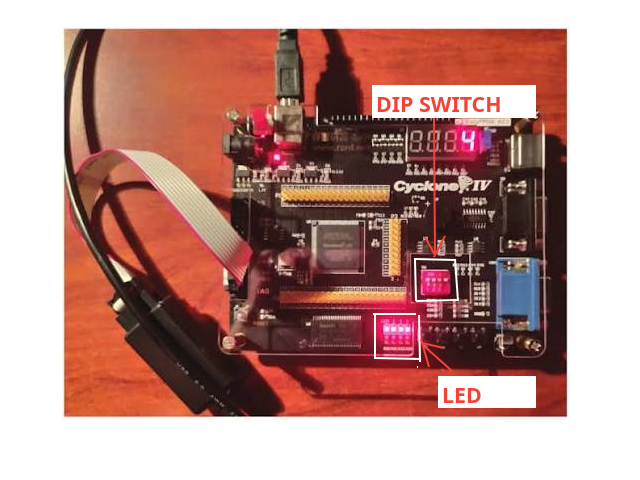
\includegraphics[width=\linewidth,height=4cm,keepaspectratio]
                {figures/dip_switch_board.png}
        }{
            \fbox{\parbox[c][4cm][c]{0.9\linewidth}{
                \centering Ảnh DIP switch trên board
            }}
        }
        \par\smallskip
        \textbf{(a)} DIP switch trên board FPGA
    \end{minipage}
    \hfill
    \begin{minipage}[b]{0.47\linewidth}
        \centering
        \IfFileExists{figures/cp2102_uart.jpg}{
            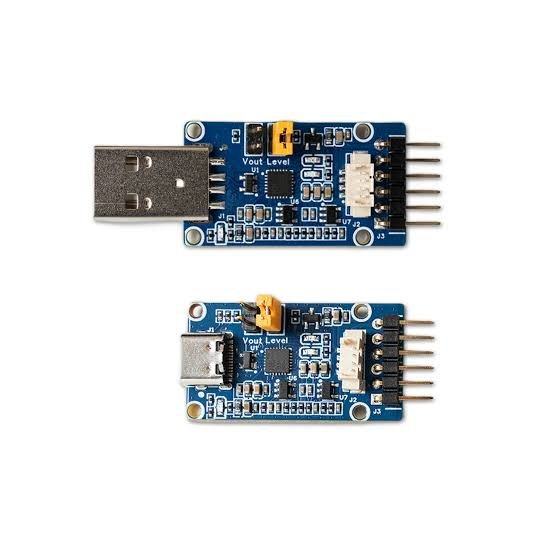
\includegraphics[width=\linewidth,height=4cm,keepaspectratio]
                {figures/cp2102_uart.jpg}
        }{
            \fbox{\parbox[c][4cm][c]{0.9\linewidth}{
                \centering Ảnh module CP2102
            }}
        }
        \par\smallskip
        \textbf{(b)} Bộ chuyển đổi USB--UART CP2102
    \end{minipage}
    \caption{Phần cứng dùng để chọn chế độ và kiểm thử giao tiếp UART.}
    \label{fig:uart_test_hardware}
\end{figure}

\begin{itemize}
    \item \textbf{Cụm công tắc DIP 
    (Hình~\ref{fig:uart_test_hardware}(a)):}
    Được sử dụng để lựa chọn chế độ kiểm tra giao tiếp UART:
    \begin{itemize}
        \item DIP1: Kiểm tra chức năng truyền dữ liệu (TX) của FPGA.
        \item DIP2: Kiểm tra chức năng nhận dữ liệu (RX) của FPGA.
        \item DIP3: Kích hoạt chế độ giao dịch dữ liệu ma trận.
    \end{itemize}

    \item \textbf{Module CP2102 
    (Hình~\ref{fig:uart_test_hardware}(b)):}
    Đóng vai trò chuyển đổi giao tiếp USB--UART giữa máy tính 
    và FPGA. Các kết nối phần cứng được thực hiện như sau:
    \begin{itemize}
        \item TXD $\rightarrow$ \texttt{uart\_rx} 
        của FPGA (\texttt{PIN\_24}).
        \item RXD $\rightarrow$ \texttt{uart\_tx} 
        của FPGA (\texttt{PIN\_114}).
        \item GND: Nối chung mass giữa module CP2102 và FPGA.
    \end{itemize}
\end{itemize}

\begin{figure}[htbp]
\centering
\resizebox{0.98\linewidth}{!}{%
\begin{tikzpicture}[
    x=1mm, y=1mm, >=stealth,
    font=\normalfont\small,
    thietbi/.style={
        draw=black!70, thick, rounded corners=1.5mm
    },
    duonggui/.style={->, thick, draw=blue!65!black},
    duongtra/.style={->, thick, draw=teal!70!black},
    dieukhien/.style={->, thick, draw=orange!55!black},
    chan/.style={font=\normalfont\ttfamily\small},
    nhan/.style={font=\normalfont\footnotesize}
]

    % Bộ chuyển đổi USB--TTL
    \path[thietbi, fill=gray!6] (19,0) rectangle (60,43);
    \node[font=\bfseries] at (39.5,37) {CP210x};
    \node at (39.5,31.5) {Bộ chuyển USB--TTL};

    % FPGA
    \path[thietbi, fill=blue!4] (110,0) rectangle (176,43);
    \node[font=\bfseries] at (143,37) {FPGA Cyclone IV E};
    \node at (143,31.5) {EP4CE6E22C8};

    % Kết nối USB với máy tính
    \node[align=center] at (6,29) {Cổng USB\\máy tính};
    \draw[<->, thick] (1,20) -- (19,20);

    % Cổng UART của CP210x
    \node[chan, anchor=east] at (59,23) {TXD};
    \node[chan, anchor=east] at (59,14) {RXD};
    \node[chan, anchor=east] at (59,5)  {GND};

    % Tên tín hiệu và số chân tương ứng trên FPGA
    \node[chan, anchor=west] at (111,23) {uart\_rx};
    \node[chan, anchor=west] at (111,14) {uart\_tx};
    \node[chan, anchor=west] at (111,5)  {GND};

    \node[chan, anchor=east] at (175,23) {PIN\_24};
    \node[chan, anchor=east] at (175,14) {PIN\_114};

    % Ba dây giữa CP210x và FPGA
    \draw[duonggui] (60,23) -- (110,23);
    \node[nhan, above] at (85,23) {Lệnh và ma trận $A$, $B$};

    \draw[duongtra] (110,14) -- (60,14);
    \node[nhan, above] at (85,14) {Phản hồi và kết quả $C$};

    \draw[thick] (60,5) -- (110,5);
    \node[nhan, above] at (85,5) {GND chung};

    % Cụm DIP trên board: mỗi cột là một công tắc
    \path[thietbi, fill=orange!8] (106,60) rectangle (180,83);
    \node[font=\bfseries] at (143,78.5) {DIP switch trên board};

    \draw[black!35] (106,74) -- (180,74);
    \draw[black!35] (131,60) -- (131,74);
    \draw[black!35] (155,60) -- (155,74);

    \node[chan] at (118.5,70) {DIP1};
    \node[nhan] at (118.5,64.5) {Thử phát TX};

    \node[chan] at (143,70) {DIP2};
    \node[nhan] at (143,64.5) {Thử nhận RX};

    \node[chan] at (167.5,70) {DIP3};
    \node[nhan] at (167.5,64.5) {Nhân ma trận};

    % Các đường chọn chế độ đi vào cạnh trên của FPGA
    \draw[dieukhien] (118.5,60) -- (118.5,43);
    \draw[dieukhien] (143,60)   -- (143,43);
    \draw[dieukhien] (167.5,60) -- (167.5,43);

    \node[fill=white, inner sep=1.5pt, font=\ttfamily\scriptsize]
        at (118.5,51.5) {PIN\_88};
    \node[fill=white, inner sep=1.5pt, font=\ttfamily\scriptsize]
        at (143,51.5) {PIN\_89};
    \node[fill=white, inner sep=1.5pt, font=\ttfamily\scriptsize]
        at (167.5,51.5) {PIN\_90};

\end{tikzpicture}%
}
\caption{Sơ đồ đấu dây UART và các công tắc chọn chế độ kiểm thử.
DIP1 kiểm tra chiều FPGA phát, DIP2 kiểm tra chiều FPGA nhận và
DIP3 kích hoạt chế độ nhân ma trận. Các công tắc tác động ở mức thấp.}
\label{fig:uart_wiring}
\end{figure}

\paragraph*{Đặc tả cơ chế hoạt động trong mỗi mode khi gạt DIP switch}

Ba công tắc DIP trên board cho phép kiểm tra lần lượt đường phát,
đường nhận và giao dịch ma trận qua UART. Khi gạt công tắc sang
vị trí ON, chân đầu vào tương ứng của FPGA ở mức logic 0.
Module \texttt{matmul.sv} đồng bộ tín hiệu theo clock 50~MHz
và lọc dội khoảng 20~ms. Nếu bộ phát đang truyền một ký tự,
hệ thống chờ đến hết stop bit trước khi đổi chế độ.

Khi nhiều công tắc cùng bật, thứ tự ưu tiên là DIP3, DIP2 rồi
DIP1. Trong quy trình kiểm thử dưới đây, mỗi lần chỉ bật một
công tắc để xác định rõ chức năng đang được kiểm tra.

\medskip
\noindent\textbf{Tất cả DIP ở OFF -- \texttt{MODE\_IDLE}.}
Đưa cả ba công tắc về OFF để kiểm tra trạng thái chờ. Các LED
báo chế độ và LED 7 đoạn đều tắt. Đường \texttt{uart\_tx} giữ
mức nghỉ logic 1. Đây cũng là chế độ ban đầu sau reset.

\begin{figure}[H]
    \centering
    \begin{subfigure}[b]{0.47\linewidth}
        \centering
        \dipimage{images/mode_idle_fsm.png}
        \caption{Điều kiện vào và ra khỏi trạng thái chờ.}
        \label{fig:mode_idle_fsm}
    \end{subfigure}
    \hfill
    \begin{subfigure}[b]{0.47\linewidth}
        \centering
        \dipimage{images/mode_idle_evidence.png}
        \caption{Trạng thái DIP và LED trên board.}
        \label{fig:mode_idle_evidence}
    \end{subfigure}
    \caption{Kiểm tra trạng thái chờ khi cả ba DIP ở OFF.}
    \label{fig:mode_idle}
\end{figure}

\noindent\textbf{Bật riêng DIP1 -- \texttt{MODE\_TX}.}
Mở terminal trên máy tính, chọn cổng của CP2102 và cấu hình
9600 baud, 8N1. Khi bật DIP1, LED1 sáng và FPGA liên tục phát
ký tự \texttt{A} (ASCII \texttt{0x41}). Sau khi hoàn tất một
khung UART, bộ phát nạp lại cùng ký tự nếu DIP1 vẫn được chọn.
Kết quả mong đợi là chuỗi \texttt{AAAA...} xuất hiện liên tục
trên cùng một dòng của terminal. Phép thử này kiểm tra chiều
từ TX của FPGA (\texttt{PIN\_114}) đến RXD của CP2102.

\begin{figure}[H]
    \centering
    \begin{subfigure}[b]{0.47\linewidth}
        \centering
        \dipimage{images/mode_tx_fsm.png}
        \caption{Trình tự nạp và phát lặp ký tự \texttt{A}.}
        \label{fig:mode_tx_fsm}
    \end{subfigure}
    \hfill
    \begin{subfigure}[b]{0.47\linewidth}
        \centering
        \dipimage{images/mode_tx_evidence.png}
        \caption{Chuỗi ký tự nhận được trên terminal.}
        \label{fig:mode_tx_evidence}
    \end{subfigure}
    \caption{Kiểm tra chiều truyền từ FPGA đến máy tính bằng DIP1.}
    \label{fig:mode_tx}
\end{figure}

\noindent\textbf{Bật riêng DIP2 -- \texttt{MODE\_RX}.}
Tắt DIP1, bật DIP2 và giữ nguyên cấu hình terminal. Trong chế độ
này, LED2 sáng. Gửi ký tự \texttt{7} từ máy tính và quan sát LED
7 đoạn trên board. Khi bộ thu nhận đủ một khung hợp lệ, tín hiệu
\texttt{rx\_valid} được kích hoạt và LED 7 đoạn hiển thị số 7.
Gửi tiếp ký tự Backspace (\texttt{0x08}) hoặc Delete
(\texttt{0x7F}) để đưa giá trị hiển thị về 0. Phép thử này kiểm
tra chiều từ TXD của CP2102 đến RX của FPGA (\texttt{PIN\_24}).

\begin{figure}[H]
    \centering
    \begin{subfigure}[b]{0.47\linewidth}
        \centering
        \dipimage{images/mode_rx_fsm.png}
        \caption{Trình tự nhận byte và cập nhật chữ số.}
        \label{fig:mode_rx_fsm}
    \end{subfigure}
    \hfill
    \begin{subfigure}[b]{0.47\linewidth}
        \centering
        \dipimage{images/mode_rx_evidence.png}
        \caption{LED 7 đoạn sau khi gửi ký tự \texttt{7}.}
        \label{fig:mode_rx_evidence}
    \end{subfigure}
    \caption{Kiểm tra chiều truyền từ máy tính đến FPGA bằng DIP2.}
    \label{fig:mode_rx}
\end{figure}

\noindent\textbf{Bật riêng DIP3 -- \texttt{MODE\_MATRIX}.}
Sau khi kiểm tra hai chiều UART bằng DIP1 và DIP2, tắt DIP2,
bật DIP3 và đóng terminal để nhường cổng nối tiếp cho GUI.
LED3 sáng, LED 7 đoạn tắt và FPGA kích hoạt bộ điều khiển
\texttt{matrix\_uart}.

Trên GUI, chọn cổng của CP2102 và nhấn \textit{Kết nối}.
Ứng dụng gửi \verb|M 0\n| để đồng bộ. Do kích thước 0 không
hợp lệ, FPGA trả \texttt{ERR} rồi \texttt{READY}; đây là phản hồi
mong đợi ở bước đồng bộ. Tiếp theo, chọn \textit{Mẫu $2\times2$}
và nhấn \textit{Gửi FPGA và đối chiếu}. Với bộ mẫu có sẵn,
giao dịch đạt khi GUI nhận đủ bốn phần tử của
\[
    C =
    \begin{bmatrix}
        19 & 22\\
        43 & 50
    \end{bmatrix},
\]
nhận dòng \texttt{READY} cuối và xác nhận kết quả FPGA khớp
với kết quả Python.

\begin{figure}[H]
    \centering
    \begin{subfigure}[b]{0.47\linewidth}
        \centering
        \dipimage{images/mode_matrix_fsm.png}
        \caption{Trình tự nhận ma trận, tính và trả kết quả.}
        \label{fig:mode_matrix_fsm}
    \end{subfigure}
    \hfill
    \begin{subfigure}[b]{0.47\linewidth}
        \centering
        \dipimage{images/mode_matrix_evidence.png}
        \caption{Kết quả FPGA và Python trên GUI.}
        \label{fig:mode_matrix_evidence}
    \end{subfigure}
    \caption{Kiểm thử giao dịch nhân ma trận bằng DIP3.}
    \label{fig:mode_matrix}
\end{figure}

Hình~\ref{fig:uart_mode_fsm} mô tả cách cập nhật thanh ghi
\texttt{mode}. Sau khi DIP ổn định, nếu bộ phát đang bận
(\texttt{tx\_busy}=1), FPGA giữ chế độ hiện tại đến hết stop bit.
Khi bộ phát rảnh, FPGA chọn chế độ theo thứ tự ưu tiên
\textbf{DIP3, DIP2, DIP1}. Vì vậy, nếu DIP1 và DIP2 cùng bật
thì FPGA chọn \texttt{MODE\_RX}; nếu DIP3 cũng bật thì FPGA chọn
\texttt{MODE\_MATRIX}.

\begin{figure}[htbp]
\centering
\resizebox{0.96\linewidth}{!}{%
\begin{tikzpicture}[
    x=1mm, y=1mm, >=stealth,
    font=\normalfont\small,
    trangthai/.style={
        draw=black!70, thick, rounded corners=2pt,
        minimum width=30mm, minimum height=11mm, align=center
    },
    mui/.style={->, thick},
    day/.style={thick},
    nhan/.style={font=\normalfont\footnotesize, align=center}
]

    % Quy tắc này áp dụng từ bất kỳ giá trị hiện tại nào của mode.
    \node[trangthai, fill=gray!8, minimum width=65mm]
        (current) at (60,40)
        {Chế độ hiện tại\\thanh ghi \texttt{mode}};

    % Nếu UART TX đang phát, giữ nguyên mode.
    \draw[mui] (current.east) -- ++(12,0)
        -- ++(0,12) -| (current.north);
    \node[nhan, above] at (83,52)
        {\texttt{tx\_busy = 1}: giữ nguyên};

    % Nếu TX rảnh, cập nhật mode theo giá trị DIP đã lọc dội.
    \draw[day] (current.south) -- (60,21);
    \node[nhan, anchor=west] at (62,28)
        {\texttt{tx\_busy = 0}};
    \draw[day] (0,21) -- (120,21);

    % Bốn trạng thái được mã hóa trong RTL.
    \node[trangthai, fill=gray!6] (idle) at (0,0)
        {\texttt{MODE\_IDLE}\\Chờ};
    \node[trangthai, fill=blue!6] (tx) at (40,0)
        {\texttt{MODE\_TX}\\Thử phát};
    \node[trangthai, fill=green!7] (rx) at (80,0)
        {\texttt{MODE\_RX}\\Thử nhận};
    \node[trangthai, fill=orange!9] (matrix) at (120,0)
        {\texttt{MODE\_MATRIX}\\Nhân ma trận};

    \draw[mui] (0,21)   -- (idle.north);
    \draw[mui] (40,21)  -- (tx.north);
    \draw[mui] (80,21)  -- (rx.north);
    \draw[mui] (120,21) -- (matrix.north);

    % Điều kiện là vị trí vật lý ON/OFF của công tắc.
    \node[nhan, fill=white] at (0,13)   {Tất cả OFF};
    \node[nhan, fill=white] at (40,13)  {Chỉ DIP1 ON};
    \node[nhan, fill=white] at (80,13)  {DIP2 ON\\DIP3 OFF};
    \node[nhan, fill=white] at (120,13) {DIP3 ON};

    % Reset đưa thanh ghi mode về IDLE.
    \draw[mui] (-24,0) -- (idle.west);
    \node[nhan, above] at (-21,0) {Reset};

\end{tikzpicture}%
}
\caption{Quy tắc chuyển giữa bốn chế độ của FPGA theo DIP switch.
Các điều kiện chuyển áp dụng từ bất kỳ chế độ hiện tại nào.}
\label{fig:uart_mode_fsm}
\end{figure}

Trình tự kiểm thử trên board là bật riêng DIP1 để kiểm tra đường
phát, bật riêng DIP2 để kiểm tra đường nhận, sau đó bật DIP3 để
chạy giao dịch ma trận hai chiều. Cả ba phép thử dùng chung cấu
hình UART được trình bày ở mục tiếp theo.

\subsubsection{Lựa chọn baud rate và cấu hình khung UART}

Trước khi kiểm tra các chế độ DIP, cấu hình cổng nối tiếp trên máy
tính ở 9600 baud, 8 bit dữ liệu, không parity, một stop bit (8N1)
và tắt điều khiển luồng. Giá trị 9600 baud được chọn để khớp với
bộ tạo thời gian bit trong hai module \texttt{uart\_tx} và
\texttt{uart\_rx} của FPGA.

Với clock $f_{\mathrm{clk}}=50$~MHz, số chu kỳ dành cho một bit
được chọn theo baud rate mục tiêu $B$:
\[
    N=\operatorname{round}\!\left(\frac{f_{\mathrm{clk}}}{B}\right),
    \qquad
    B_{\mathrm{thực}}=\frac{f_{\mathrm{clk}}}{N}.
\]
Với $B=9600$, ta có $N=5208$. Trong RTL, bộ đếm chạy từ 0 đến
\texttt{BIT\_LAST = 5207}, tương ứng đúng 5208 chu kỳ cho mỗi bit.
Bộ thu dùng \texttt{HALF\_LAST = 2603} để lấy mẫu gần giữa bit.
Ba thông số thời gian thu được là
\[
    B_{\mathrm{thực}}\approx 9600{,}61~\mathrm{baud},\qquad
    T_{\mathrm{bit}}=104{,}16~\mu\mathrm{s},\qquad
    T_{\mathrm{8N1}}=10T_{\mathrm{bit}}=1{,}0416~\mathrm{ms}.
\]

Khi giữ nguyên clock 50~MHz, tăng $N$ làm mỗi bit kéo dài hơn và
baud rate giảm. Chẳng hạn, để chuyển sang 19200 baud, cần đặt
$N=2604$, đổi \texttt{BIT\_LAST} thành 2603 ở cả bộ phát và bộ thu,
đổi \texttt{HALF\_LAST} thành 1301 ở bộ thu, đồng thời cập nhật
baud rate trên máy tính. Các lựa chọn về parity và stop bit quyết
định số bit trong một khung, do đó ảnh hưởng thời gian truyền một
ký tự. Trong thiết kế 8N1 hiện tại, mỗi ký tự gồm một start bit,
tám bit dữ liệu và một stop bit.

\subsubsection{Kiểm tra đường phát bằng DIP1}

Bật riêng DIP1 và mở terminal nối tiếp ở cấu hình 9600 baud, 8N1.
Ở chế độ này, FPGA liên tục phát ký tự \texttt{A} có mã ASCII
\texttt{0x41}. Khi bộ phát rảnh, \texttt{uart\_tx} nạp ký tự vào
thanh ghi phát. Sau khi phát hết stop bit, bộ phát tiếp tục nạp
ký tự kế tiếp nếu DIP1 vẫn được chọn.

\begin{figure}[htbp]
\centering
\resizebox{0.87\linewidth}{!}{%
\begin{tikzpicture}[
    x=1mm,y=1mm,>=stealth,
    st/.style={draw,rounded corners=2pt,fill=blue!6,
               minimum height=9mm,align=center},
    arr/.style={->,thick}
]
    \node[st] (idle) at (0,0) {Chờ chọn DIP1};
    \node[st] (load) at (48,0) {Nạp \texttt{0x41}};
    \node[st] (send) at (98,0) {Phát khung 8N1};

    \draw[arr] (idle) -- node[above,font=\scriptsize]{DIP1 bật} (load);
    \draw[arr] (load) -- (send);
    \draw[arr] (send.south) -- ++(0,-10)
        -| node[pos=.25,below,font=\scriptsize]
        {Hết stop bit, DIP1 còn bật} (load.south);
    \draw[arr] (send.north) -- ++(0,10)
        -| node[pos=.25,above,font=\scriptsize]
        {Hết khung, tắt DIP1} (idle.north);
\end{tikzpicture}%
}
\caption{Trình tự phát lặp ký tự \texttt{A} khi kiểm tra riêng DIP1.}
\label{fig:uart_dip1_tx}
\end{figure}

Kết quả mong đợi là terminal hiển thị liên tục \texttt{AAAA...}
trên cùng một dòng. Phép thử này kiểm tra đường từ
\texttt{uart\_tx} của FPGA tại \texttt{PIN\_114} đến RXD của CP210x.
Nếu terminal hiển thị ký tự sai, kiểm tra lại baud rate và định dạng
khung trước khi chuyển sang thử chiều nhận.

\subsubsection{Kiểm tra đường nhận bằng DIP2}

Tắt DIP1, bật riêng DIP2 và giữ nguyên cấu hình terminal. Gửi ký tự
\texttt{7} từ máy tính. Dữ liệu đi từ TXD của CP210x đến
\texttt{uart\_rx} tại \texttt{PIN\_24}. Khi nhận được một khung hợp
lệ, bộ thu phát xung \texttt{rx\_valid}; mạch hiển thị dùng byte vừa
nhận để cập nhật LED 7 đoạn.

\begin{figure}[htbp]
\centering
\resizebox{0.92\linewidth}{!}{%
\begin{tikzpicture}[
    x=1mm,y=1mm,>=stealth,
    st/.style={draw,rounded corners=2pt,fill=green!7,
               minimum height=9mm,align=center},
    arr/.style={->,thick}
]
    \node[st] (wait) at (0,0) {Chờ byte hợp lệ};
    \node[st] (show) at (71,11) {Hiển thị chữ số};
    \node[st] (clear) at (71,-11) {Đưa hiển thị về 0};

    \draw[arr] (wait.north east) --
        node[above,sloped,font=\scriptsize]
        {ASCII \texttt{0} đến \texttt{9}} (show.west);
    \draw[arr] (wait.south east) --
        node[below,sloped,font=\scriptsize]
        {Backspace hoặc Delete} (clear.west);

    \draw[arr] (show.north) -- ++(0,8) -| (wait.north);
    \draw[arr] (clear.south) -- ++(0,-8) -| (wait.south);
\end{tikzpicture}%
}
\caption{Xử lý byte nhận trong chế độ DIP2. Các ký tự khác giữ
nguyên chữ số đang hiển thị.}
\label{fig:uart_dip2_rx}
\end{figure}

LED 7 đoạn phải hiển thị số 7. Nhấn Enter thì số 7 vẫn giữ nguyên;
gửi Backspace (\texttt{0x08}) hoặc Delete (\texttt{0x7F}) thì
màn hình trở về 0. Việc quan sát trực tiếp trên board xác nhận FPGA
đã nhận đúng byte từ máy tính.

\subsubsection{Kiểm thử phép nhân ma trận bằng DIP3}

Sau khi DIP1 xác nhận chiều FPGA phát và DIP2 xác nhận chiều FPGA
nhận, bật riêng DIP3 để kiểm tra hai chiều trong cùng một giao dịch.
Đóng terminal để giải phóng cổng nối tiếp, sau đó mở GUI và chọn
đúng cổng. Ở chế độ này, LED3 sáng và LED 7 đoạn tắt.

\begin{figure}[htbp]
\centering
\resizebox{0.97\linewidth}{!}{%
\begin{tikzpicture}[
    x=1mm,y=1mm,>=stealth,
    st/.style={draw,rounded corners=2pt,fill=orange!9,
               minimum height=10mm,align=center},
    arr/.style={->,thick}
]
    \node[st] (ready) at (0,0) {Phát \texttt{READY}\\và chờ lệnh};
    \node[st] (recv)  at (42,0) {Nhận kích thước\\và ma trận $A,B$};
    \node[st] (run)   at (85,0) {Nạp bộ nhân\\và tính $C$};
    \node[st] (reply) at (125,0) {Phát ma trận $C$\\qua UART};

    \draw[arr] (ready) -- node[above,font=\scriptsize]{\texttt{M}} (recv);
    \draw[arr] (recv) -- node[above,font=\scriptsize]{Đủ dữ liệu} (run);
    \draw[arr] (run) -- node[above,font=\scriptsize]{Hoàn tất} (reply);
    \draw[arr] (reply.south) -- ++(0,-10)
        -| node[pos=.25,below,font=\scriptsize]
        {Đã gửi hàng cuối} (ready.south);
    \draw[arr] (recv.north) -- ++(0,10)
        -| node[pos=.25,above,font=\scriptsize]
        {Dữ liệu lỗi: phát \texttt{ERR}} (ready.north);
\end{tikzpicture}%
}
\caption{Các giai đoạn của một giao dịch ma trận khi bật DIP3.}
\label{fig:uart_dip3_matrix}
\end{figure}

Khi kết nối, GUI gửi \verb|M 0\n| để đồng bộ. Do kích thước 0
không hợp lệ, FPGA đi theo nhánh lỗi trong
Hình~\ref{fig:uart_dip3_matrix}, phát \texttt{ERR} rồi
\texttt{READY}. Đây là phản hồi mong đợi ở bước đồng bộ.
Tiếp theo, chọn mẫu $2\times2$ và nhấn
\textit{Gửi FPGA và đối chiếu}. Phép thử đạt khi GUI nhận đủ
bốn phần tử của $C$, nhận dòng \texttt{READY} cuối và xác nhận
từng giá trị khớp với kết quả Python.

\subsection{Giao diện nạp ma trận, tính toán và đọc kết quả}

\subsubsection{Giao diện trên máy tính}

Giao diện được viết bằng PyQt5 trong tệp \texttt{matrix\_gui.py}.
Người dùng chọn ba kích thước $M$, $K$, $N$, sau đó nhập ma trận
$A_{M\times K}$ và $B_{K\times N}$. Mỗi hàng được nhập trên một
dòng, các phần tử phân cách bằng khoảng trắng. Mỗi kích thước nhận
giá trị từ 1 đến 8. Đối với bài toán chính của đề tài, chọn
$M=K=N=8$.

\begin{figure}[htbp]
    \centering
    \includegraphics[width=0.94\linewidth]{figures/matrix_gui_2x2.png}
    \caption{Giao diện với bộ mẫu $2\times2$. Hai ô phía trên chứa
    ma trận đầu vào. Ở thời điểm chụp, GUI đã tính kết quả Python
    và đang ở trạng thái chưa kết nối FPGA.}
    \label{fig:uart_matrix_gui}
\end{figure}

\begin{itemize}
    \item \textbf{Kết nối và đồng bộ.}
    Sau khi người dùng chọn cổng và nhấn \textit{Kết nối}, GUI gửi
    \verb|M 0\n|. Kích thước 0 khiến FPGA trả hai dòng \texttt{ERR}
    rồi \texttt{READY}. GUI nhận đúng thứ tự này để xác nhận phiên
    làm việc đã đồng bộ. Thời hạn chờ là 5 giây.

    \item \textbf{Tính kết quả tham chiếu.}
    Nút \textit{Tính Python} kiểm tra số hàng, số cột và miền giá trị
    $[-32768,32767]$ của từng phần tử, sau đó hiển thị
    $C_{\mathrm{ref}}=A\cdot B$. Chức năng này có thể sử dụng trước
    khi kết nối board.

    \item \textbf{Gửi và đối chiếu.}
    Nút \textit{Gửi FPGA và đối chiếu} tính lại $C_{\mathrm{ref}}$
    từ dữ liệu hiện tại rồi gửi yêu cầu qua UART. Khi nhận đủ ma trận
    $C$ và dòng \texttt{READY} cuối, GUI so sánh từng ô. Nếu có sai
    lệch, giao diện hiển thị số ô sai, tọa độ ô sai đầu tiên và hai
    giá trị tương ứng. Thời hạn chờ giao dịch là 15 giây.
\end{itemize}
\subsubsection{Định dạng dữ liệu và ví dụ giao dịch}

Sau khi chuyển sang chế độ DIP3 và đồng bộ với FPGA, GUI gửi yêu cầu
nhân ma trận dưới dạng văn bản ASCII. Dòng đầu bắt đầu bằng ký tự
lệnh \texttt{M} (mã \texttt{0x4D}), theo sau là ba kích thước
$M$, $K$, $N$ của phép nhân $A_{M\times K}B_{K\times N}$.
Tiếp theo, GUI gửi $M K$ phần tử của $A$ rồi đến $K N$ phần tử
của $B$, theo thứ tự từng hàng. Hai số trên cùng một hàng được
phân cách bằng dấu cách và mỗi hàng kết thúc bằng ký tự LF
(\texttt{0x0A}).

FPGA phân biệt dữ liệu của hai ma trận bằng số phần tử đã nhận.
Sau khi ghi đủ $M K$ phần tử vào RAM $A$, bộ điều khiển tự chuyển
sang nhận $B$. Vì vậy, GUI chỉ gửi giá trị các phần tử trong phần
dữ liệu. Ký tự \texttt{A} phát lặp ở chế độ DIP1 chỉ dùng để kiểm
tra đường truyền từ FPGA đến máy tính.

\begin{figure}[htbp]
    \centering
    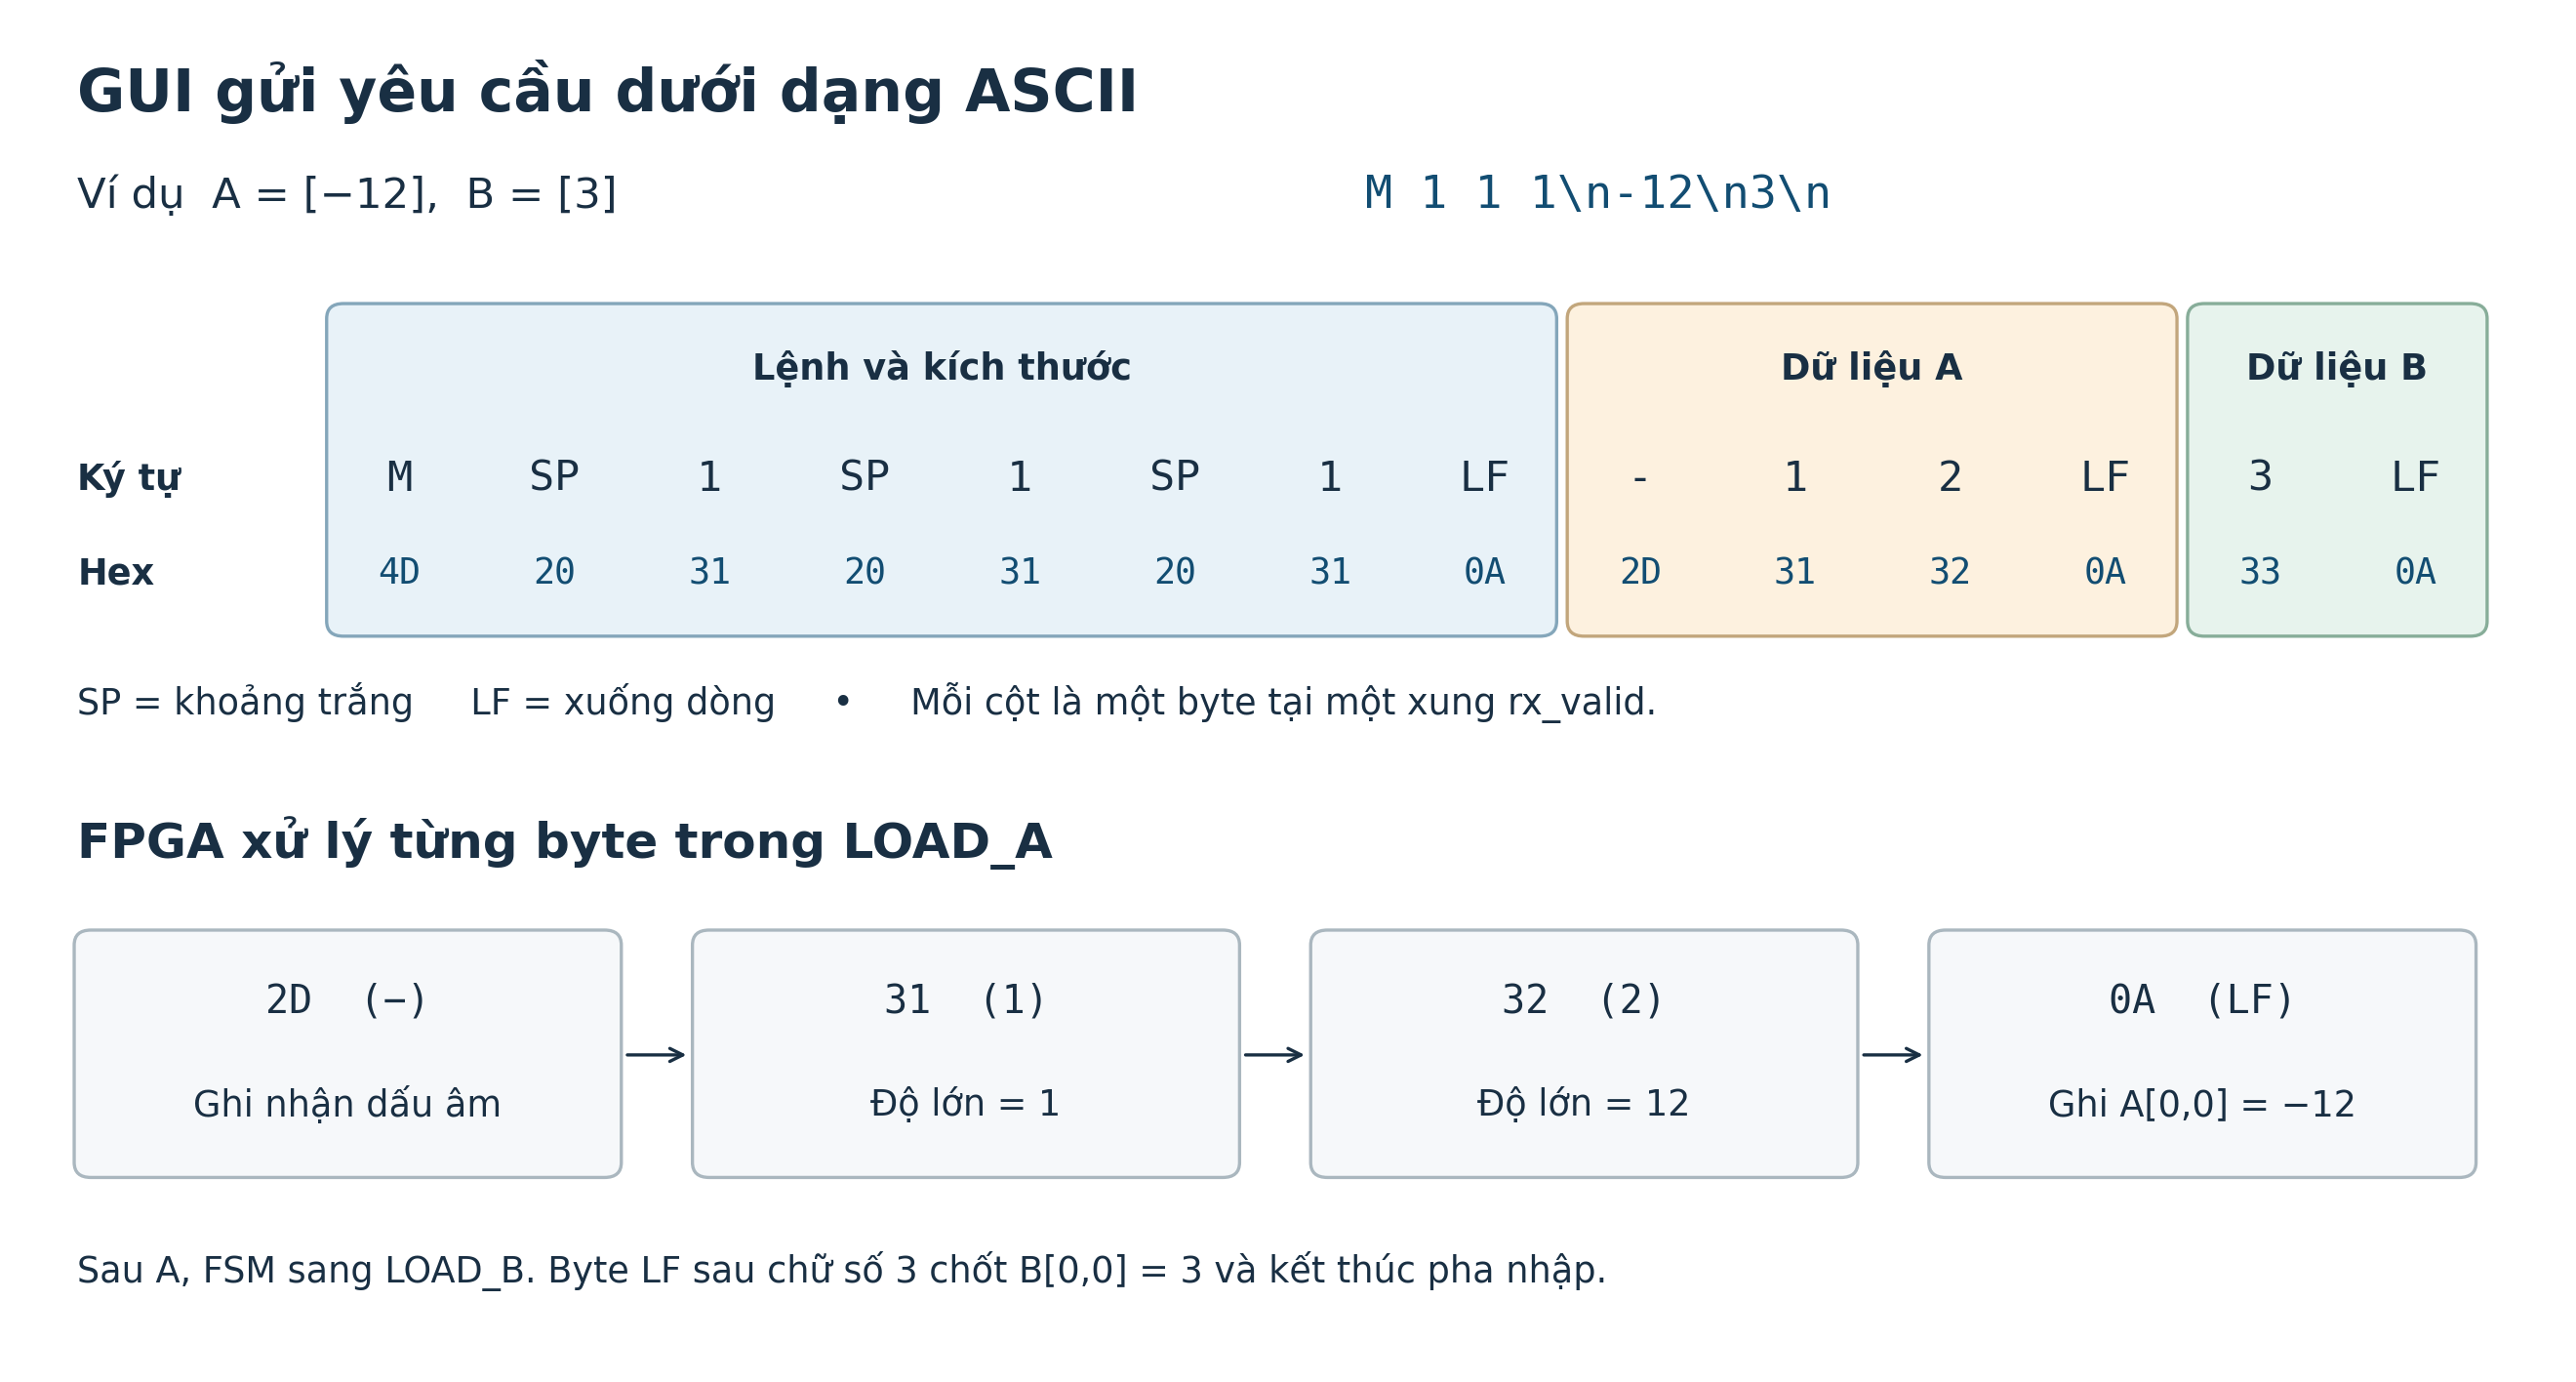
\includegraphics[width=0.98\linewidth]{figures/uart_ascii_parser.png}
    \caption{Giải mã bản tin ASCII cho $A=[-12]$ và $B=[3]$.
    Mỗi cột biểu diễn một byte. SP là dấu cách và LF là ký tự xuống dòng.}
    \label{fig:uart_ascii_parser}
\end{figure}

Trong Hình~\ref{fig:uart_ascii_parser}, GUI gửi chuỗi
\verb|M 1 1 1\n-12\n3\n| gồm 14 byte. Mỗi cụm \verb|\n| trong
cách viết này biểu diễn một byte LF. Riêng phần tử $-12$ cần ba
ký tự ASCII để biểu diễn giá trị và một ký tự LF để chốt số:

\begin{itemize}
    \item \texttt{0x2D} là dấu trừ. Bộ giải mã ghi nhận số đang
    nhập có dấu âm.
    \item \texttt{0x31} và \texttt{0x32} là các chữ số 1 và 2.
    Với mỗi chữ số $d$, bộ giải mã cập nhật độ lớn theo
    $v\leftarrow 10v+d$. Giá trị $v$ lần lượt bằng 1 rồi bằng 12.
    \item \texttt{0x0A} kết thúc số. Bộ điều khiển áp dụng dấu
    và ghi $-12$ vào RAM $A$ dưới dạng số bù hai 16 bit
    (\texttt{0xFFF4}). Hai byte tiếp theo, \texttt{0x33} và
    \texttt{0x0A}, chốt giá trị 3 vào RAM $B$.
\end{itemize}

Bảng~\ref{tab:uart_example} trình bày giao dịch của bộ mẫu
$2\times2$ trên GUI theo thứ tự thời gian.

\begin{table}[htbp]
\centering
\caption{Trình tự trao đổi UART khi nhân hai ma trận $2\times2$}
\label{tab:uart_example}
\small
\begin{tabularx}{\linewidth}{@{}l l X@{}}
\toprule
\textbf{Chiều truyền} & \textbf{Dòng ASCII} & \textbf{Ý nghĩa} \\
\midrule
PC $\to$ FPGA & \texttt{M 2 2 2} & Lệnh nhân với $M=K=N=2$. \\
PC $\to$ FPGA & \texttt{1 2}     & Hàng đầu của $A$. \\
PC $\to$ FPGA & \texttt{3 4}     & Hàng cuối của $A$. \\
PC $\to$ FPGA & \texttt{5 6}     & Hàng đầu của $B$. \\
PC $\to$ FPGA & \texttt{7 8}     & LF sau số 8 chốt phần tử cuối của $B$. \\
\midrule
FPGA $\to$ PC & \texttt{C 2 2}   & Kết quả có hai hàng và hai cột. \\
FPGA $\to$ PC & \texttt{19 22}   & Hàng đầu của $C$. \\
FPGA $\to$ PC & \texttt{43 50}   & Hàng cuối của $C$. \\
FPGA $\to$ PC & \texttt{READY}   & Kết thúc giao dịch, sẵn sàng nhận lệnh mới. \\
\bottomrule
\end{tabularx}
\end{table}

Chẳng hạn, giá trị 19 ở hàng kết quả đầu tiên tương ứng với
$C_{0,0}=1\times5+2\times7$. Mỗi dòng do FPGA phát kết thúc bằng
CR/LF (\texttt{0x0D}, \texttt{0x0A}). GUI kiểm tra kích thước,
nhận đủ hai hàng và chờ dòng \texttt{READY} cuối trước khi đối
chiếu bốn phần tử với kết quả Python.

\subsubsection{Trình tự xử lý trong FPGA}

Module \texttt{uart\_rx} tiếp nhận khung 8N1 và xuất một byte trên
\texttt{rx\_data}. Khi stop bit hợp lệ, tín hiệu \texttt{rx\_valid}
lên mức 1 trong một chu kỳ clock. Bộ điều khiển
\texttt{matrix\_uart} sử dụng xung này để xử lý từng ký tự theo
trạng thái hiện tại của FSM.

\begin{enumerate}
    \item \textbf{Giải mã lệnh và ghi RAM đầu vào.}
    Từ \texttt{WAIT\_M}, ký tự lệnh đưa FSM sang
    \texttt{DIM\_M}, \texttt{DIM\_K} rồi \texttt{DIM\_N} để nhận
    ba kích thước. Trong \texttt{LOAD\_A} và \texttt{LOAD\_B},
    FSM ghép các chữ số như minh họa ở
    Hình~\ref{fig:uart_ascii_parser}. Khi gặp dấu phân cách sau
    một số hợp lệ, FSM ghi phần tử vào địa chỉ $8r+c$, với $r,c$
    là chỉ số hàng và cột tính từ 0. Trên waveform,
    \texttt{rx\_valid} đánh dấu một byte vừa nhận, còn
    \texttt{accept\_token} trong trạng thái nạp đánh dấu thời điểm
    phần tử được ghi vào RAM.

    \item \textbf{Đóng gói dữ liệu và khởi chạy bộ nhân.}
    Sau khi chốt phần tử cuối của $B$, FSM lần lượt thực hiện
    \texttt{TILE\_READ}, \texttt{TILE\_PACK} và \texttt{TILE\_LOAD}.
    Bốn phần tử 16 bit tạo thành một gói 64 bit. Bộ điều khiển nạp
    16 gói cho $A$ rồi 16 gói cho $B$; các ô ngoài kích thước yêu
    cầu được điền 0. Tại \texttt{CORE\_START}, bộ nhân nhận lệnh
    khi \texttt{core\_start\_ready} bằng 1. Cả hai kiến trúc dùng
    cùng giao diện nạp này; bên trong lõi baseline, một MAC vẫn
    xử lý lần lượt từng phần tử.

    \item \textbf{Thu kết quả nhị phân.}
    Trong \texttt{CORE\_WAIT}, mỗi cạnh clock có
    \texttt{core\_result\_valid} bằng 1 tương ứng với một lần ghi
    kết quả 35 bit vào RAM $C$ tại địa chỉ do bộ nhân cung cấp.
    Do lõi xử lý khung $8\times8$, bộ điều khiển thu đủ 64 giá trị,
    kể cả khi GUI yêu cầu phép nhân $2\times2$. Khi nhận
    \texttt{core\_done}, FSM chuyển sang \texttt{HEADER}.

    \item \textbf{Định dạng và phát phản hồi.}
    FSM phát dòng kích thước \texttt{C} kèm $M$, $N$, rồi đọc
    $M\times N$ phần tử cần trả từ RAM $C$. Đối với mỗi phần tử,
    FSM lưu dấu, chuyển trị tuyệt đối sang BCD trong 35 chu kỳ
    và phát từng chữ số ASCII qua \texttt{uart\_tx}. Dấu trừ
    được phát trước chữ số nếu giá trị âm. Sau hàng cuối, FPGA
    gửi dòng \texttt{READY} để kết thúc giao dịch.
\end{enumerate}

\paragraph{Mốc đo khi kiểm thử.}
Trong ca mô phỏng \texttt{FINAL\_1\_UART\_8x8} của kiến trúc
multicast ở 50~MHz, mốc hoàn tất nhập liệu là cạnh clock tại đó
\texttt{accept\_token} chốt phần tử cuối trong \texttt{LOAD\_B}.
Từ mốc này, hệ thống mất 290 chu kỳ để nạp dữ liệu và đưa bộ nhân
đến cạnh nhận \texttt{start}, sau đó mất thêm 121 chu kỳ để nhận đủ
64 kết quả. Như vậy, thời gian từ khi chốt đầu vào đến khi RAM $C$
của \texttt{matrix\_uart} có đủ kết quả là
\[
    (290+121)\times20~\mathrm{ns}
    = 411\times20~\mathrm{ns}
    = 8{,}220~\mu\mathrm{s}.
\]
Riêng khoảng từ \texttt{start} đến lần nhận kết quả thứ 64 là
$2{,}420~\mu\mathrm{s}$. Khi đo toàn bộ giao dịch trên đường UART,
từ start bit đầu của yêu cầu đến hết stop bit của byte LF cuối
trong dòng \texttt{READY}, kết quả là $607{,}214$~ms đối với bộ
dữ liệu này. Thời gian toàn giao dịch phụ thuộc số ký tự ASCII
cần truyền, bao gồm chữ số, dấu âm và ký tự phân cách.